\documentclass[notitlepage]{revtex4-1}
% includes...
\usepackage{amsmath}
\usepackage{bm}
\usepackage{natbib}
\usepackage{graphicx}
\usepackage{hyperref}
\usepackage{epstopdf}
\usepackage{color}

\begin{document}
%front matter
\title{SUNSET-code documentation}

\author{J. R. C. King}
\email{jack.king@manchester.ac.uk}
\affiliation{School of Engineering, The University of Manchester, UK}
\date{\today}
\begin{abstract}
This document details the governing equations and numerical methods used in the \textbf{S}calable \textbf{U}nstructured \textbf{N}ode-\textbf{SET} code (aka. SUNSET code), and provides brief instructions for configuration and running of the code.

\end{abstract}

\maketitle
%end front matter

\section{Introduction}

This document describes the \textbf{S}calable \textbf{U}nstructured \textbf{N}ode-\textbf{SET} code (aka. SUNSET code). The code is designed for direct numerical simulations of compressible turbulent reacting flows in non-trivial geometries. It builds on the work in~\cite{king_2020,king_2022}, using the Local Anisotropic Basis Function Method (LABFM) for spatial discretisation, combined with high-order finite differences in the third dimension, and a third-order Runge-Kutta time integration. This guide should be read in conjunction with the preprint~\cite{king_2024}.

\subsection{Key features at a glance:}
\begin{itemize}
\item Solves the fully compressible multi-species reacting Navier-Stokes equations, with detailed chemistry, on an unstructured node-set.
\item Resolution may be non-uniform in space, including along boundaries.
\item Spatial discretisation uses LABFM in the $x_{1}-x_{2}$ plane, combined with high-order finite differences in the (homogeneous) third dimension $x_{3}$.
\item High-order (up to $10^{th}$) discretisation in space dropping to $4^{th}$ order at boundaries.
\item $3^{rd}$ order explicit Rungke-Kutta time integration with adaptive error control.
\item Boundary conditions using NSCBC: (non-reflecting) inflows \& outflows, isothermal or adiabatic walls.
\item Periodic/symmetry/low-order-wall boundaries also available.
\item Written in \verb|Fortran 90|, accelerated with MPI \& OpenMP.
\end{itemize}


\subsection{A comment on notation}

Subscripts $i$, $j$, and $k$ are vector indices for Einstein notation, and for these indices, repetition implies summation. Subscripts $\alpha$ and $\beta$ indicate chemical species. Subscripts $a$ and $b$ indicate collocation point indices. Subscripts $l$ and $L$ are used for polynomial coefficient indices. Subscript $m$ is for chemical reaction number (regular-size $m$ is polynomial order). Note that this is consistent with~\cite{king_2024}, but not~\cite{king_2020,king_2022}, in which we used $i$ and $j$ to indicate collocation point indices.

\section{The Governing Equations}\label{ge}

The code solves the compressible Navier-Stokes equations in conservative form
\begin{subequations}\begin{align}
\frac{\partial\rho}{\partial{t}}+\frac{\partial\rho{u}_{k}}{\partial{x}_{k}}=&~0\label{eq:mass}\\
\frac{\partial\rho{u}_{i}}{\partial{t}}+\frac{\partial\rho{u}_{i}u_{k}}{\partial{x}_{k}}=&-\frac{\partial{p}}{\partial{x}_{i}}+\frac{\partial\tau_{ki}}{\partial{x}_{k}}+\rho{f}_{i}\label{eq:mom}\\
\frac{\partial\rho{E}}{\partial{t}}+\frac{\partial\rho{u}_{k}E}{\partial{x}_{k}}=&-\frac{\partial{p}u_{k}}{\partial{x}_{k}}-\frac{\partial{q}_{k}}{\partial{x}_{k}}+\frac{\partial\tau_{ki}u_{i}}{\partial{x}_{k}}+\rho\displaystyle\sum_{\alpha}Y_{\alpha}f_{k}\left({u}_{k}-V_{\alpha,k}\right)\label{eq:en}\\
\frac{\partial\rho{Y}_{\alpha}}{\partial{t}}+\frac{\partial\rho{u}_{k}Y_{\alpha}}{\partial{x}_{k}}=&~\dot\omega_{\alpha}-\frac{\partial\rho{V}_{\alpha,k}Y_{\alpha}}{\partial{x}_{k}}\qquad\forall\alpha\in\left[1,N_{S}\right]\label{eq:Y}
\end{align}
\end{subequations}
where $\rho$ is the density, ${u}_{i}$ the $i$-th component velocity, $p$ the pressure, $E$ the total energy, $\tau$ the viscous stress, $f$ a body force, $q$ the heat flux, $Y_{\alpha}$ the concentration of species $\alpha\in\left[1,N_{S}\right]$, and $V_{\alpha,k}$ is the $k$-th component of the molecular diffusion velocity of species $\alpha$. $\dot\omega_{\alpha}$ is the production rate of species $\alpha$.

The viscous stress is defined as 
\begin{equation}\tau_{ki}=\mu\left(\frac{\partial{u}_{k}}{\partial{x}_{i}}+\frac{\partial{u}_{i}}{\partial{x}_{k}}-\frac{2}{3}\frac{\partial{u}_{j}}{\partial{x}_{j}}\delta_{ik}\right)\label{eq:tau},\end{equation}
where $\mu$ is the dynamic viscosity and $\delta_{ik}$ is the Kronecker delta. The energy is
\begin{equation}E=\displaystyle\sum_{\alpha}h_{\alpha}Y_{\alpha}-\frac{p}{\rho}+\frac{1}{2}{u}_{i}{u}_{i}\label{eq:E}\end{equation}
where the sum over $\alpha$ is over all $\alpha\in\left[1,N_{S}\right]$, and $h_{\alpha}$ is the enthalpy of species $\alpha$. The molecular diffusion term in~\eqref{eq:Y} is modelled as a Fickian diffusion process with
\begin{equation}-\rho{V}_{\alpha,k}Y_{\alpha}=\rho\hat{V}_{\alpha,k}Y_{\alpha}-Y_{\alpha}\displaystyle\sum_{\beta\in\left[1,N_{S}\right]}\rho\hat{V}_{\beta,k}Y_{\beta}\label{eq:fickdiff},\end{equation}
in which $\rho\hat{V}_{\alpha,k}Y_{\alpha}$ is obtained from the diffusion model (either constant Lewis numbers or mixtured-averaged), and the final term is a correction to ensure that 
\begin{equation}\displaystyle\sum_{\alpha}Y_{\alpha}=1.\label{eq:sumY}\end{equation}
The heat flux vector is then given by
\begin{equation}q_{k}=-\lambda\frac{\partial{T}}{\partial{x}_{k}}+\displaystyle\sum_{\alpha}\rho{V}_{\alpha,k}Y_{\alpha}h_{\alpha}\label{eq:hfv},\end{equation}
where $\lambda$ is the thermal conductivity of the mixture.
The system is closed with an ideal gas equation of state
\begin{equation}\frac{p}{\rho}={R}_{mix}T=\frac{R_{0}T}{W_{mix}}={R}_{0}T\displaystyle\sum_{\alpha}\frac{Y_{\alpha}}{W_{\alpha}}\label{eq:eos}\end{equation}
where $R_{mix}$ is the gas constant for the mixture, $R_{0}$ is the universal gas constant, and $W_{\alpha}$ is the molar mass of species $\alpha$, and $W_{mix}$ is the molar mass of the mixture.

\subsection{Evaluation of temperature and heat capacity}

The temperature dependence of the specific heat capacity of species $\alpha$ is given by a polynomial of order $L$
\begin{equation}c_{p,\alpha}=\displaystyle\sum_{l=1}^{L}a_{\alpha,l}T^{l-1},\end{equation}
which is valid over a specified temperature range $T\in\left[T_{low},T_{high}\right]$, and in which the coefficients $a_{\alpha,l}$ are constructed to fit the standard NASA polynomials~\cite{gordon_1971}. Integration of this yields an expression for the enthalpy
\begin{equation}h_{\alpha}=\displaystyle\sum_{l=1}^{L}\frac{a_{\alpha,l}}{l}T^{l} + a_{\alpha,L+1},\end{equation}
whilst the temperature derivative of $c_{p,\alpha}$ is
\begin{equation}\frac{dc_{p,\alpha}}{dT}=\displaystyle\sum_{l=1}^{L}\left(l-1\right)a_{\alpha,l}T^{l-2}.\end{equation}
Noting that the specific heat capacity of species $\alpha$ is $R_{0}/W_{\alpha}$, where $R_{0}$ is the universal gas constant and $W_{\alpha}$ is the molar mass of species $\alpha$, the energy can be written as
\begin{equation}E=\displaystyle\sum_{\alpha}Y_{\alpha}\left(h_{\alpha}-R_{0}\frac{T}{W_{\alpha}}\right)+\frac{1}{2}\bm{u}\cdot\bm{u}.\end{equation}
Substituting the polynomial for $h_{\alpha}$ and collecting terms in powers of $T$, we can write
\begin{equation}f\left(T\right)=C_{0}+\displaystyle\sum_{l=1}^{L}C_{l}T^{l}=0,\label{eq:nonlinearT}\end{equation}
where the coefficients $C$ are given by
\begin{subequations}\begin{align}
C_{0}&=\frac{1}{2}\bm{u}\cdot\bm{u}-E+\displaystyle\sum_{\alpha}Y_{\alpha}a_{\alpha,L+1}\\
C_{1}&=\displaystyle\sum_{\alpha}Y_{\alpha}a_{\alpha,1} - R_{mix}\\
C_{l}&=\displaystyle\sum_{\alpha}Y_{\alpha}\frac{a_{\alpha,l}}{l}\qquad\forall{l}\in\left[2,L\right].\end{align}\end{subequations}
The derivative of $f$ is
\begin{equation}f^{\prime}\left(T\right)=\displaystyle\sum_{l=1}^{L}lC_{l}T^{l-1}.\end{equation}
Having calculated the coefficients $C$, we solve the nonlinear equation~\eqref{eq:nonlinearT} numerically via a Newton-Raphson method to obtain the temperature $T$.

Note that in the case where $a_{\alpha,1}\ne0$ and $a_{\alpha,l\in\left[2,L\right]}=0$ (i.e. $c_{p,\alpha}$ is independent of temperature), $f\left(T\right)$ is linear in $T$, and the Newton-Raphson method will converge (exactly) after a single iteration.

\subsection{Transport properties}

Two models are implemented for transport properties. The constant Lewis number approximation, and a mixture averaged transport model.

\subsubsection{Constant Lewis numbers}

In this model, the diffusive flux is given by
\begin{equation}\rho\hat{V}_{\alpha,k}Y_{\alpha}=-\rho{D}_{\alpha}\frac{\partial{Y}_{\alpha}}{\partial{x}_{k}},\end{equation}
in which $D_{\alpha}$ is the molecular diffusivity of species $\alpha$. The temperature dependence of transport properties is modelled by the relationship
\begin{equation}\mu=\mu_{ref}\left(\frac{T}{T_{ref}}\right)^{r_{T}},\label{eq:tdtp_mu}\end{equation}
where $\mu_{ref}$ is the viscosity at the reference temperature $T_{ref}$, and $r_{T}=0.7$ is a constant exponent. The mixture thermal conductivity is given by
\begin{equation}\lambda=\frac{\mu{c}_{p}}{Pr},\end{equation}
in which $c_{p}$ is the heat capacity of the mixture, and $Pr$ is the Prandtl number, taken as constant. The molecular diffusivity of species $\alpha$ is given by
\begin{equation}D_{\alpha}=\frac{\lambda}{\rho{c}_{p}Le_{\alpha}},\end{equation}
where $Le_{\alpha}$ is the Lewis number for species $\alpha$, which is assumed constant for each species.

\subsubsection{Mixtured-averaged transport}

In this model the diffusive flux is given by 
\begin{equation}\rho\hat{V}_{\alpha,k}Y_{\alpha}=-\rho{D}_{\alpha}\frac{\partial{Y}_{\alpha}}{\partial{x}_{k}}-\rho{D}_{\alpha}Y_{\alpha}\left(\frac{\partial\ln{T}}{\partial{x}_{k}}+\frac{\partial\ln\rho}{\partial{x}_{k}}-\frac{W_{\alpha}}{\rho{R}_{0}T}\frac{\partial{p}}{\partial{x}_{k}}\right),\end{equation}

Here the transport properties for individual species and species pairs are evaluated using standard polynomial fits~\cite{kee_1986}
\begin{subequations}\begin{align}
\ln\mu_{\alpha}&=\displaystyle\sum_{l=1}^{L}c_{\mu,\alpha,l}\left(\ln\left(\frac{T}{T_{ref}}\right)\right)^{l-1}\\
\ln\lambda_{\alpha}&=\displaystyle\sum_{l=1}^{L}c_{\lambda,\alpha,l}\left(\ln\left(\frac{T}{T_{ref}}\right)\right)^{l-1}\\
\ln{D}_{\alpha\beta}&=\ln\left(\frac{p_{ref}}{p}\right)+\displaystyle\sum_{lj=1}^{L}c_{D,\alpha\beta,l}\left(\ln\left(\frac{T}{T_{ref}}\right)\right)^{l-1},
\end{align}\end{subequations}
in which the $c_{\dots,l}$ are constants, and $L=4$. The transport properties are then obtained from combination rules following~\cite{ern_1994,ern_1995} as
\begin{equation}\mu=\left[\displaystyle\sum_{\alpha}X_{\alpha}\mu_{\alpha}^{n_{\mu}}\right]^{\frac{1}{n_{\mu}}},\end{equation}
with $n_{\mu}=6$, 
\begin{equation}\lambda=\left[\displaystyle\sum_{\alpha}X_{\alpha}\lambda_{\alpha}^{n_{\lambda}}\right]^{\frac{1}{n_{\lambda}}},\end{equation}
with $n_{\lambda}=1/4$, and the combination rule for molecular diffusivity follows the Hirschfelder-Curtiss approximation~\cite{hirschfelder_curtiss}
\begin{equation}D_{\alpha}=\frac{\displaystyle\sum_{\beta\ne\alpha}X_{\beta}{W}_{\beta}}{W_{mix}\displaystyle\sum_{\beta\ne\alpha}\frac{X_{\beta}}{D_{\alpha\beta}}}.\end{equation}
Note that the molar concentration $X_{\alpha}=Y_{\alpha}W_{mix}/W_{\alpha}$.
Soret and Dufour effects are neglected.

\subsection{Evaluation of reaction rates}

The reaction mechanism is given by $M$ equations written in the form
\begin{equation}\displaystyle\sum_{\alpha}\nu_{\alpha,m}^{\prime}\mathcal{M}_{\alpha}\rightarrow\displaystyle\sum_{\alpha}\nu_{\alpha,m}^{\prime\prime}\mathcal{M}_{\alpha}\qquad\forall{m}\in\left[1,M\right],\end{equation}
where $\mathcal{M}_{\alpha}$ symbolises the chemical symbol of species $\alpha$, and 
$\nu_{\alpha,m}^{\prime}$ and $\nu_{\alpha,m}^{\prime\prime}$ are the molar stoichiometric coefficients of species $\alpha$ in equation $m$.

The reaction rate of species $\alpha$ is given by
\begin{equation}\omega_{\alpha}=W_{\alpha}\displaystyle\sum_{m=1}^{M}\hat{\omega}_{\alpha,m}\end{equation}
where $\hat{\omega}_{\alpha,m}$ is the molar production rate of species $\alpha$ due to the $m$-th reaction, and $M$ is the total number of reactions. The molar production rates are given by
\begin{equation}\hat{\omega}_{\alpha,m}=\left(\nu^{\prime\prime}_{\alpha,m}-\nu^{\prime}_{\alpha,m}\right)\left[k_{f,m}\left(T\right)\displaystyle\prod_{\beta=1}^{N_{S}}\left(\frac{\rho{Y}_{\beta}}{W_{\beta}}\right)^{\nu^{\prime}_{\beta,m}}-k_{b,m}\left(T\right)\displaystyle\prod_{\beta=1}^{N_{S}}\left(\frac{\rho{Y}_{\beta}}{W_{\beta}}\right)^{\nu^{\prime\prime}_{\beta,m}}\right],\end{equation}
in which $k_{f,m}$ and $k_{b,m}$ are the forward and backward (respectively) rate constants for reaction $m$. The forward rate constant is given by the Arrhenius expression
\begin{equation}k_{f,m}\left(T\right)=A_{m}T^{n_{m}}\exp\left(-\frac{E_{a,m}}{R_{0}T}\right),\end{equation}
with $A_{m}$, $n_{m}$ and $E_{a,m}$ being specified constants representing the pre-exponential factor, the temperature dependence of the pre-exponential factor, and the activation energy.

\subsubsection{Backwards rate constant}

The backwards rate constant is related to the forward rate constant via
\begin{equation}\ln{k}_{b,m}=\ln{k}_{f,m} + \displaystyle\sum_{\alpha}\left(\nu^{\prime\prime}_{\alpha,m}-\nu^{\prime}_{\alpha,m}\right)\left(\frac{\hat{g}_{\alpha}}{R_{0}T}+\ln\left(\frac{P_{0}}{R_{0}}\right)-\ln{T}\right),\end{equation}
in which $P_{0}$ is a reference pressure, and $\hat{g}_{\alpha}$ is the Gibbs function for species $\alpha$, which is given by
\begin{equation}\frac{\hat{g}_{\alpha}}{W_{\alpha}T}=\frac{a_{\alpha,J+1}}{T}-a_{\alpha,1}\ln{T}+\left(a_{\alpha,1}-a_{\alpha,J+2}\right)-\displaystyle\sum_{j=2}^{J}\frac{a_{\alpha,j}}{j\left(j-1\right)}T^{j-1},\end{equation}
with the coefficients again following the standard NASA polynomials~\cite{gordon_1971}.

\subsubsection{Third bodies}

For a step $m$ including third bodies $\mathcal{M}$, reaction rates are scaled by the third-body concentration $c_{M,m}$, which is given by
\begin{equation}c_{M,m}=\displaystyle\sum_{\alpha}\eta_{\alpha,m}\frac{\rho{Y}_{\alpha}}{W_{\alpha}},\end{equation}
and $\eta_{\alpha,m}$ are the third-body efficiencies for species $\alpha$ for step $m$.

\subsubsection{Lindemann forms}

Where the Arrhenius form is insufficient to describe the reaction rate, a pressure (partial pressure/concentration) dependancy is introduced, and the forward reaction rate takes the Lindemann form:
\begin{equation}k_{f,m}=k_{\infty,m}\left(\frac{P_{r}}{1+P_{r}}\right)F_{m},\end{equation}
where $F_{m}$ is the Troe fall-off rate, and a constant for steps with Lindemann form. $P_{r}$ is a reduced pressure given by
\begin{equation}P_{r}=\frac{k_{0,m}}{k_{\infty,m}},\end{equation}
$k_{0,m}$ is the Arrhenius rate of the reaction, and $k_{\infty,m}$ is a second Arrhenius rate. Hence for Lindemann steps, in addition to the three Arrhenius coefficients, the constant $F_{m}$ is prescribed, along with the pre-exponential factor, the temperature dependence of the pre-exponential factor and the activation energy for $k_{\infty,m}$. Note that after evaluation of the rate constants for Lindemann steps, the third-body concentration of the step is reset to unity. Steps with non-constant Troe fall-off rate are not yet implemented.

\section{The Numerical Methods}\label{ni}

The spatial discretisation is based on the Local Anisotropic Basis Function Method (LABFM) in the first two dimensions, and high-order finite differences in the third dimension. LABFM has been detailed and extensively analysed in~\cite{king_2020,king_2022}, and the present implementation is described in~\cite{king_2024} and we refer the reader to these works for a complete description.

To summarise, the domain is discretised in the $x_{1}-x_{2}$ plane with an unstructured point cloud of $N_{12}$ nodes. The discretisation in the third dimension is uniform: there are $N_{3}$ copies of each node in the $x_{1}-x_{2}$ plane, equispaced along the $x_{3}$ axis. Hence, there are a total of $N=N_{12}N_{3}$ nodes in the domain. Each node $a\in\left[1,N\right]$ has position $x_{a,i}$, a distribution lengthscale $s_{a}$, and a computational stencil lengthscale $h_{a}$. $s_{a}$ is the average node spacing around node $a$, and is analagous to the grid spacing in a finite difference scheme. The spacing in $x_{3}$ is denoted $s_{3}$, and is uniform throughout the domain, whilst $s_{a}$ can vary as a function of $x_{1}$ and $x_{2}$. Each node holds the conservative variables $\rho_{a}$, $\rho{u}_{i,a}$, $\rho{E}_{a}$ and $\rho{Y}_{\alpha,a}$. The governing equations are solved on the set of $N$ nodes. 

The difference between properties at two nodes is denoted $\left(\cdot\right)_{ba}=\left(\cdot\right)_{b}-\left(\cdot\right)_{a}$. The computational stencil for each node $a$ is denoted $\mathcal{N}_{a}$, and is constructed to contain all nodes $b$ in the same $x_{1}-x_{2}$ plane such that $\lvert{x}_{i,ba}x_{i,ba}\rvert\le4h_{a}^{2}$, (with the repeated subscript $i$ implying summation), alongside all the nodes with $x_{1,ba}=x_{2,ba}=0$ required to build a finite difference stencil in the $x_{3}$ dimension. The unstructured nodes in the $x_{1}-x_{2}$ plane are created to fill the domain using a variation of the propagating front algorithm of~\cite{fornberg_2015a}, following~\cite{king_2022}.

\subsection{Evaluation of spatial derivatives}

Spatial derivative operators take the form
\begin{equation}L^{d}_{a}\left(\cdot\right)=\displaystyle\sum_{b}\left(\cdot\right)_{ba}w^{d}_{ba},\label{eq:general_do}\end{equation}
where $d$ identifies the derivative of interest (e.g. $d=x_{1}$ indicates the operator $L^{d}$ approximates $\partial\left(\cdot\right)/\partial{x}_{1}$, and $d=x_{i}x_{i}$ (summation implied) indicates the operator approximates the Laplacian), and $w^{d}_{ba}$ are a set of inter-node weights for the operator. Note that the construction of~\eqref{eq:general_do} takes the same form for both LABFM-based and finite difference-based derivative approximations. For derivatives in the $x_{3}$ dimension, the weights $w^{d}_{ba}$ are simply central finite difference weights of order $m$. For derivatives in the $x_{1}-x_{2}$ plane, LABFM is used to set the $w^{d}_{ba}$, which is constructed from a weighted sum of anisotropic basis functions centred on node $a$. The basis functions used herein are formed from bi-variate Hermite polynomials multiplied by a radial basis function, and the basis function weights are set such that the operator achieves a specified polynomial consistency $m$. Calculation of these weights is done as a pre-processing step, and described in detail in~\cite{king_2022}. 

The order of the spatial discretisation can be specified between $m=4$ and $m=10$, but is set by default to $m=8$ uniformly away from boundaries. This provides a good compromise between accuracy and computational cost. At non-periodic boundaries, the consistency of the LABFM reconstruction is smoothly reduced to $m=4$. The stencil scale $h_{a}$ is initialised to $h_{a}=2.7s_{a}$ in the bulk of the domain, and $h_{a}=2.4s_{a}$ near boundaries (choices informed through experience as being large enough to ensure stability). In bulk of the domain, the stencil scale is then reduced following the optimisation procedure described in~\cite{king_2022}. This has the effect of both reducing computational costs, and increasing the resolving power of LABFM, yielding the smallest stencil size $h_{a}$ for which the discretisation remains stable.

The evaluation of derivatives using~\eqref{eq:general_do} constitutes the bulk of the computational cost, and it is hence desirable only use it where essential, and where possible to use analytic expressions to relate derivatives of secondary properties to those evaluated via~\eqref{eq:general_do}. First derivatives of $\rho$, ${u}_{i}$, $\rho{E}$ and ${Y}_{\alpha}$, alongside the temperature $T$ and pressure $p$, are evaluated directly using~\eqref{eq:general_do}. Convective terms are then constructed from combinations thereof: for example
\begin{equation}\frac{\partial\rho{u}_{i}E}{\partial{x}_{i}}=u_{i}\frac{\partial\rho{E}}{\partial{x}_{i}}+\rho{E}\frac{\partial{u}_{i}}{\partial{x}_{i}}.\end{equation}
Laplacians and direct second (i.e. $\partial^{2}\left(\cdot\right)/\partial{x}_{i}\partial{x}_{i}$) derivatives are also evaluated with~\eqref{eq:general_do}. To avoid the explicit evaluation of cross-second derivatives of velocity, the viscous stress divergence is evaluated as
\begin{equation}\frac{\partial\tau_{ki}}{\partial{x}_{k}}=\frac{1}{\mu}\frac{\partial\mu}{\partial{x}_{k}}\tau_{ki}+\mu\left(\frac{\partial^{2}{u}_{i}}{\partial{x}_{k}\partial{x}_{k}}+\frac{1}{3}\frac{\partial^{2}{u}_{k}}{\partial{x}_{i}\partial{x}_{k}}\right)\label{eq:divtau},\end{equation}
where the final term is the gradient of the velocity divergence, which is calculated through two iterations of first derivative evalations with~\eqref{eq:general_do}. The benefit of this approach is that it reduces the stencil size, and provides a significant reduction in the complexity associated with parallelising the scheme. Gradients of secondary properties are evaluated from analytic expressions in terms of gradients of primary properties. The gradient of the enthalpy of species $\alpha$ is given by
\begin{equation}\frac{\partial{h}_{\alpha}}{\partial{x}_{k}}=\frac{dh_{\alpha}}{dT}\frac{\partial{T}}{\partial{x}_{k}}=c_{p,\alpha}\frac{\partial{T}}{\partial{x}_{k}},\end{equation}
and the gradient of the mixture specific heat capacity is
\begin{equation}\frac{\partial{c}_{p}}{\partial{x}_{k}}=\displaystyle\sum_{\alpha}\left[Y_{\alpha}\frac{dc_{p,\alpha}}{dT}\frac{\partial{T}}{\partial{x}_{k}}+c_{p,\alpha}\frac{\partial{Y}_{\alpha}}{\partial{x}_{k}}\right].\end{equation}
When constant Lewis numbers are assumed, additional relations are available to evaluate the spatial derivatives of transport properties:
\begin{equation}\frac{\partial\mu}{\partial{x}_{k}}=\frac{r_{T}\mu}{T}\frac{\partial{T}}{\partial{x}_{k}}\end{equation}
\begin{equation}\frac{\partial\lambda}{\partial{x}_{k}}=\frac{r_{T}\lambda}{T}\frac{\partial{T}}{\partial{x}_{k}}+\frac{\lambda}{c_{p}}\frac{\partial{c_{p}}}{\partial{x}_{k}}\end{equation}
\begin{equation}\frac{\partial\rho{D}_{\alpha}}{\partial{x}_{k}}=\frac{r_{T}D_{\alpha}}{T}\frac{\partial{T}}{\partial{x}_{k}}.\end{equation}
For the mixture averaged model, gradients of $\mu$, $\lambda$ and $\rho{D}_{\alpha}$ are obtained directly using~\eqref{eq:general_do}.

\subsection{Temporal integration and filtering}

The governing equations are integrated in time using a four-step third-order, low-storage explicit Runge-Kutta scheme, with embedded second order error estimation, denoted RK3(2)4[2R+]C in the classification system of~\citet{kennedy_2000}. The value of the time step is set adaptively using a PID controller to keep time-integration errors below a specified threshold, set to $10^{-4}$ as a default. The solution is de-aliased after each time-step by high-order spatial filtering using the filters described in~\cite{king_2022} combined with a finite difference filter following~\cite{kennedy_1994}. Details of the filtering procedure can be found in~\cite{king_2024}.


\subsection{Boundaries}

For full details of the implementation of boundaries we refer the reader to~\cite{king_2022,king_2024}. To summarise, the node distribution is locally structured at the boundaries, in the vicinity of which derivative operators are constructed from combinations of LABFM and asymmetric finite differences. Numerical boundary conditions are imposed through the Navier-Stokes Characteristic Boundary Condition formalism, details of which can be found in~\cite{poinsot_2005,sutherland_2003,yoo_2007}. For walls and hard inflows, we follow the procedures described in~\cite{poinsot_2005}. For non-reflecting outflows we follow the approach of~\cite{sutherland_2003}. For non-reflecting inflows we use the \emph{improved} formulation of~\cite{yoo_2007}.

\subsection{Parallelisation}

The code is accelerated with MPI and OpenMP, and uses a static non-uniform block-structured three-dimensional domain decomposition. The distributed parallelism with MPI scales extremely well ($>96\%$ from $4$ to $1024$ MPI ranks). The shared parallelism is limited by memory access competition, and scales very poorly - improvements are in the pipeline here. For now, we use $1$ thread, and the code is hard-coded to use only $1$ thread by default.

In the $x_{1}$ and $x_{3}$ directions, periodic boundary conditions are imposed through the MPI structure, whilst in the $x_{2}$ direction they are imposed locally on each MPI rank. Communications are blocking, and due to the cyclical structure for any domain periodicity, \textbf{an even number of MPI ranks is required in each direction}.


\section{The Code}

There are currently four branches of the code, which are becoming increasingly divergent, but they are summarised as follows:
\begin{enumerate}
\item \verb|main| - the main branch which solves the equations above in dimensional form for multistep chemistry.
\item \verb|nondim| - this branch solves for single-step chemistry in entirely non-dimensional form.
\item \verb|oned| - this is a one-dimensional version which is suitable for quickly simulating laminar flames to generate input files for the main branch.
\item \verb|ev| - solves the isothermal Navier-Stokes equations for a single species, along with a constitutive equation for viscoelastic flows. This branch is unrelated to combustion. Details of the equations and formulations for this branch can be found in~\cite{king_2023}.
\end{enumerate}

Check github regularly for the most up to date versions. Please do not directly modify any of the above branches (especially main). Create a new branch to work on, and we will merge developments into \verb|main| later.

\subsection{Directory structure}

The code is in a directory called \verb|sunset_code|, and has a structure as follows:
\begin{itemize}
\item \verb|data_out| - contains
\begin{itemize}
\item files called \verb|nodesxxxxx|, where \verb|xxxxx| is equal to $10000$ plus the processor number associated with that node file. (e.g. the nodes file saved by processor $4$ is called \verb|nodes10003|).
\item files called \verb|fieldsxxxxx_xxx|, where \verb|xxxxx| again indicates the processor, and \verb|_xxx| gives the number of the output (e.g. \verb|fields10003_123| is the $123^{rd}$ output of the $4^{th}$ processor.
\item \verb|time.out|, which lists the output fields files and the number of nodes in each file.
\item a directory \verb|statistics| which contains a set of files holding the temporal variation of various global statistics. 
\end{itemize}
\item \verb|docs| - contains this document and associated latex files.
\item \verb|obj| - contains the object/mod files generated on compilation.
\item \verb|paraview_files| - holds .vtu files (once produced by the code in \verb|vtk_conv|) which can be loaded into Paraview.
\item \verb|runfiles| - contains subdirectories each holding template control files for various levels of chemistry.
\item \verb|restart| - contains files needed to restart the simulation from a previous run.
\item \verb|source| - contains the source code for the main program in directories \verb|base| and \verb|common|, and source code used to generate input discretisations in \verb|gen| and \verb|ishift|.
\item \verb|vtk_conv| - contains a small code written in Fortran which converts the \verb|fieldsxxxxx_xxx| into .vtu files in the \verb|paraview_files| directory.
\end{itemize}

\subsection{Code structure}

The code has a modular stucture, with each module (each file in \verb|source/base/|) containing routines which perform similar operations, or which perform operations in a similar context. For example, routines which evaluate spatial derivatives are located in \verb|source/base/derivatives.F90|, and routines which evaluation thermodynamic quantities (e.g. $T$ from $\rho{E}$, $\rho{u}_{i}$ and $Y_{\alpha}$, or $c_{p}$ from $T$) are contained within \verb|source/base/thermodynamics.F90|.

At the high level, the code has the following structure. The main program is in \verb|source/base/sunset.F90|, which
\begin{itemize}
\item Calls routines to setup the domain, domain decomposition, LABFM and FD operators, and initial/restart conditions.
\item Initialises value of time-step $\delta{t}$, then starting at $t=0$, loops whilst $t<t_{max}$
\begin{itemize}
\item Calls output routines if it is the correct time to output data
\item Calls routines to evaluate the time-step $\delta{t}$.
\item Calls a routine in \verb|source/base/step.F90| which conducts one full RK time step, consisting of
\begin{itemize}
\item Calling routines in \verb|source/base/rhs.F90| to evaluate the RHS of the equations
\item Integrating forward one RK substep
\item Re-applying BCs
\item MPI communications
\item Repeating the above 4 steps for all RK substeps
\item Filtering the solution
\item Re-applying BCs
\item MPI communications
\end{itemize}
\end{itemize}
\item Cleans up and ends the simulation.
\end{itemize}

The routines in \verb|source/base/rhs.F90| call other routines to evaluate thermodynamic and transport properties, derivatives, chemical source terms, and characteristic boundary conditions.

\subsection{Prerequisites}

The code is largely free of dependencies on external libraries, with the exception of \verb|openblas|, which is used for solving the local consistency matrices for LABFM. An in-house SVD routine has been tested and implemented for systems where \verb|openblas| is not available, but the performance is better with \verb|openblas|, and the SVD routine is not included by default.

It also requires a system with \verb|gfortran| (for non-MPI runs, and compilation of the codes in \verb|vtk_conv|, \verb|source/gen/| and \verb|source/ishift|), \verb|mpifort| (for MPI runs), and the OpenMP libraries. These requirements should be trivial to satisfy for most Unix systems. For other compilers, modify the \verb|Makefile| as required.

\section{Running the code}

\subsection{Generating the discretisation}

The first step in running the code is to generate a node discretisation for the desired geometry. This is done by navigating to \verb|source/gen/|, modifying \verb|datclass.F90|, compiling it (just use \verb|make|), and running it (using \verb|.gen2D|). This little code has a number of cases (e.g. doubly periodic, periodic channel, simple flame-tube, inflow-outflow with obstacle/bluff body) which you can choose at runtime. More can be added. Changing geometry and parameters controlling the resolution etc is done by hard-coding and recompiling for each case. This code uses the propagating front algorithm (which some tweaks) of~\cite{fornberg_2015a} to generate the distribution. See Appendix~\ref{ap:datclass} for more (important) details.


The next step is to prepare the discretisation for the main \verb|sunset-code|. To do this, navigate to \verb|source/ishift/| and compile the code herein (use \verb|make|). First, run \verb|./ishift| and enter $1$ at the prompt. This will perform $50$ iterations of a simple shifting procedure, which makes the node distribution slightly smoother and better suited to LABFM.

Next re-run the \verb|./ishift|, but at the prompt enter $0$. The next prompts will request the number of MPI processors in the $x$, $y$ and $z$ (i.e. $x_{1}$, $x_{2}$ and $x_{3}$ directions). For 2D simulations choose $1$ for the number in $z$. In general, if the number of processors in any direction is not equal to $1$, it should be \textbf{even}. Otherwise there is a risk the code will get stuck on a blocking MPI communication and just hang. For example, to run a two-dimensional simulation with $24$ MPI processors, we would run \verb|./ishift|, then enter $0$, $6$, $4$, $1$.

Note that care must be taken to ensure the number of processors in any direction is not too large for the resolution in that direction. For the above example with a $6$ by $4$ decomposition schedule, if the domain is a very long narrow flame-tube, the sub-domains will be too narrow (smaller than the computational stencil), and the \verb|sunset_code| will crash. The code \verb|ishift| provides a warning if the decomposition schedule is likely to result in MPI domains which are too small, but it is not foolproof. In general, for domains with significantly varying resolution, it is harder to find a decomposition schedule which doesn't cause these problems.

With the above steps complete, a file called \verb|IPART| will be placed in the main directory. This file contains the decomposition schedule and a list of all the nodes, and is read in by \verb|sunset_code| at the start of the simulation.

\subsection{Control}

The simulation is then controlled by three files, all with the suffix \verb|.in|: \verb|control.in|, \verb|thermochem.in| and \verb|transport.in|. These contain the main control parameters, the thermochemistry of the fluids being simulated, and the transport properties (respectively). The latter two are less likely to require editing.

Clean copies of all three files are located within the sub-directories of \verb|runfiles/| for the different chemistries available. Note, formatting of these files is sensitive: if you add an erroneous blank line to any of these files, \verb|sunset_code| will read it incorrectly.

The parameters in \verb|control.in| are largely self-explanatory, but more detail will be added to this document in due course. 

\subsubsection{Setting the initial flow field}

This is partially controlled by \verb|control.in|, for example in the specification of a base-flow profile (zero, uniform or parabolic), the choice of flow type (e.g. flame, Gaussian hot-spot, loading a flame file), and coordinates/scales of initial flames. The routines which implement the initial flow state are in~\verb|source/base/setup_flow.F90|, and the routines which implement error-function based flame profiles, Gaussian hotspots, density stratification etc can be modified as required.

\subsection{Running from initial conditions}

\begin{itemize}
\item Run the above steps to generate \verb|IPART|
\item Copy the control files from the appropriate sub-directory with \verb|runfiles| and modify as required.
\item Modify \verb|source/base/setup_flow.F90| to specify the required initial conditions.
\item Compile sunset code using (e.g.) \verb|make react=1|
\item Run the code on the correct number of processors using (e.g.) \verb|mpirun -n 24 ./sunset|
\end{itemize}

\subsection{Running from a restart file}

\begin{itemize}
\item Copy \verb|data_out/nodes*| to \verb|restart/.|.
\item Copy \verb|data_out/*xxx| to \verb|restart/.|, where xxx indicates the number of the output file from which you wish to restart.
\item Within \verb|restart|, run \verb|sh fnm_strip.sh| $a+1$ times, where $a$ is the number of digits in xxx above. This removes the underscore and all subsequent characters from the \verb|fieldsxxxxx_xxx| filenames, ready for the code to load them on restart. e.g. if you're restarting from output file $xxx=123$, run \verb|sh fnm_strip.sh| $4$ times. 
\item If the previous run was a restart, you're ready to go. Otherwise, store any output files you wish to save, then in the main directory, \verb|make clean|, then (e.g.) \verb|make react=1 restart=1|.
\item Run the code, using (e.g.) \verb|mpirun -n 8 ./sunset|
\end{itemize}

Note that the file \verb|IPART| in the main directory for a restarted run needs to be the same (exactly the same) as the one used for the original run. It is not (at present) possible to change the decomposition schedule between original and restarted runs.

\subsection{Screen output}

If running the code interactively (i.e. not via a grid-engine/jobscript/queue system), it is best to use a terminal $80\times{24}$ characters. Every $100$ time-steps the screen will be updated with information on the simulation, including maxima and minima for density, velocity, pressure and temperature, the time-step, and some information on profiling and performance.

\appendix

\section{Details on generating a discretisation}\label{ap:datclass}

Within each case in \verb|datclass.F90| there are several steps. Figure~\ref{fig:case7} shows a snippet of code for an example case, of a porous geometry (an array of cylinders) with inflow and outflow conditions. Running through the case in order, we have:
\begin{itemize}
\item Lines $195$ to $200$: specifying the domain size \verb|xl| and \verb|yl|, and other lengthscales relevant to the geometry. In this case \verb|D_cyl| is the cylinder diameter, \verb|S_cyl| is the cylinder spacing, \verb|h0| is the cylinder radius, and \verb|dx0| is the \emph{baseline} resolution.
\item Line $201$: specifying the non-NSCBC boundaries with \verb|xbcond| and \verb|ybcond|. Values of $1$, $2$ and $3$ indicate periodic, symmetry and low-order walls respectively. A value of $0$ is used where the boundary is going to be set by the NSCBC (i.e. for isothermal/adiabatic walls, or inflow/outflow conditions).
\item Lines $203$ to $210$: Creating the outer geometry. The domain is a rectangle, defined by $4$ boundary patches connection the $4$ nodes specified in lines $207$ to $210$. The entries in the array \verb|b_type| define the type of boundary on the respective patch. Values of $0$, $1$ and $2$ indicate isothermal/adiabatic walls, inflows, and outflows respectively. A value of $3$ indicates the non-NSCBC boundary conditions defined by \verb|xbcond| and \verb|ybcond| are to be used. In this example, the first and third patches (lower and upper) have periodic conditions, whilst the second (right) and fourth (left) are outflow and inflow respectively.
\item Lines $211$ to $231$: define a set of \emph{blobs} which are the solid obstacles making up the porous media. Each blob is defined by the coordinates of its centre \verb|blob_centre|, a set of coefficients \verb|blob_coeffs|, and a rotation \verb|blob_rotation|. The shape of the blob is then defined in polar coordinates (about the its centre) as
\begin{equation}r_{blob}\left(\theta\right)=\displaystyle\sum_{n=1}^{\verb|n_blob_coefs|}a_{n}cos\left(2\pi{n}\left(\theta+\theta_{0}\right)\right),\end{equation}
where the $a_{n}$ are the blob-coefficients, $\theta_{0}$ is the blob rotation, and $r_{blob}$ and $\theta$ are the polar coordinates with origin at the blob centre. This construction can be used to make quite a variety of shapes, provided a) the centre of area lies within the blob (i.e. no horseshoes), and b) the maximum curvature of the blob surface can be resolved by the resolution. I have a Matlab script which generates coefficients, and has been tested for rounded edge squares, triangles, and aerofoils. In the present example, the blobs are circular, so $\verb|blob_coeffs|=\verb|h0|,0,0,0\dots$.
\item Lines $233$ and $234$: specify the resolution variation (within the hard-coded constraints). \verb|dxmin| is the smallest resolution in the domain, and is automatically used at blob surfaces. \verb|dx_wall|, \verb|dx_in| and \verb|dx_out| are the resolutions at walls, inflows and outflows on the outer geometry. There are some contrivances in this section - it has not been well automated - and for some cases additional scaling factors are included to (e.g.) stretch regions of fine resolution where a flame is likely to occur.
\end{itemize}

\subsection{Troubleshooting}

If after running \verb|gen2D| you run \verb|ishift| and get a segmentation fault (often stating an index of \verb|ij_count| is out of range), it's likely the discretisation generated by \verb|gen2D| needs modifying. The (current) best approach is to generate a discretisation with \verb|gen2D|, run \verb|ishift| twice, then run \verb|sunset-code| and use paraview to visualise the first output file.

\begin{figure}
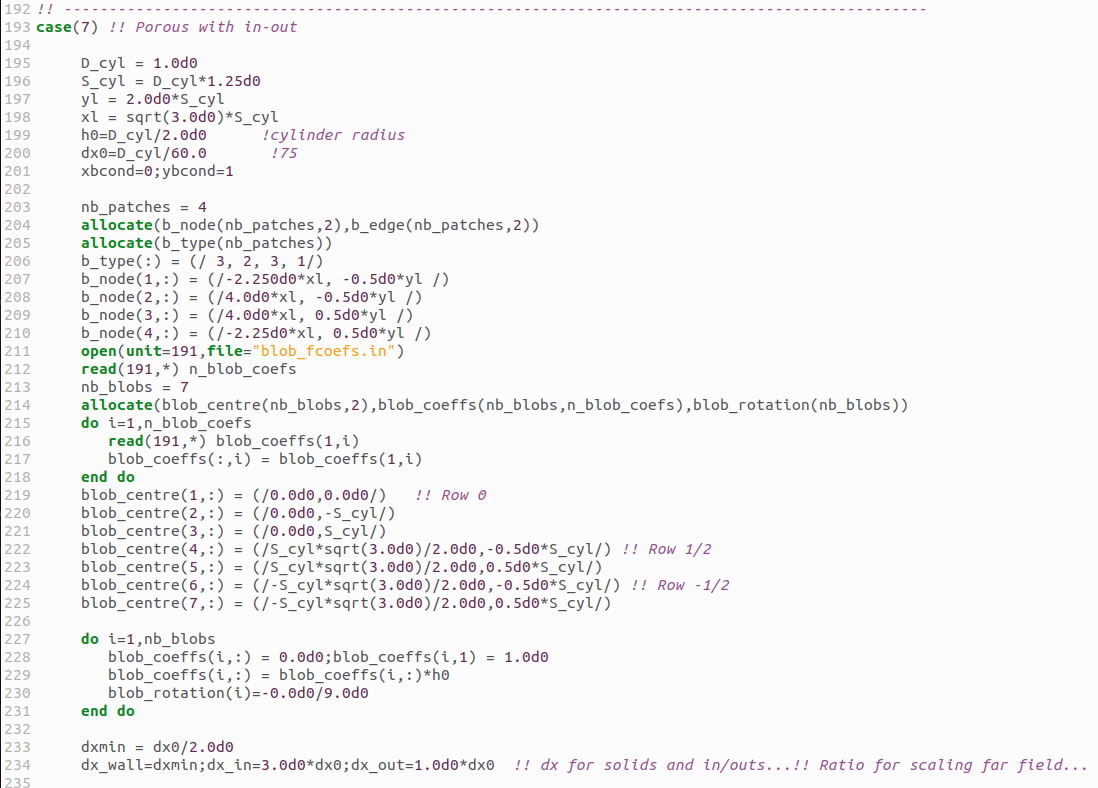
\includegraphics[width=0.9\textwidth]{case7.png}
\caption{Code snippet for an example case.\label{fig:case7}}
\end{figure}


%\bibliographystyle{elsarticle-num-names}
\bibliography{jrckbib}

\end{document}


